% !TeX spellcheck = en_GB
\chapter{The \Jiben{} \Jianfa{}}\label{ch:jianfa}

The term \Jiben{} \Jianfa{} (\begin{CJK*}{UTF8}{bsmi}基本劍法\end{CJK*}) denotes what is generally referred to as the sword basic techniques or basic cuts.
It may be translated literally as: the \textit{basic}, \textit{elementary}, \textit{fundamental} (\Jiben{}) \textit{methods} (\Fa{}), of the \textit{straight sword} (\Jian{}).

The different styles of \Taijijian{} report a variable number of \Jiben{} \Jianfa{}, usually ranging from four to thirteen or more. The names of several of them are mentioned already in the \JianJing{}, a sword treatise written by \YuDayou{} around 1560, or in the \WubeiZhi{}, a military encyclopaedia presumably published in 1620.
It is not clear though whether these terms were already referring to the very same techniques as they do today in \Taijijian{}, and even more so as the \Jiben{} \Jianfa{} names are not always consistent across styles.

The \Yangjia{} \Michuan{} \Taijijian{} tradition lists eight \Jiben{} \Jianfa{}, each corresponding to one of the eight sections in the \Kunlun{} sword form: \Pi{}, \Ci{}, \Liao{}, \Zha{}, \Mo{}, \Duo{}, \Tiao{}, \Hua{}.
A ninth one, \Dian{}, is also referred to, but is sometimes described as a combination of \Pi{} and \Ci{}, possibly in order to preserve the fit total number of eight pure techniques.
Whatever the reason for it, I have the feeling that this description of \Dian{} as a combination actually acknowledges that the \Jiben{} \Jianfa{} can be mixed together.
I therefore like to consider them not as techniques \textit{per se} but rather as technical principles that, blended together, make up the actual sword techniques. The so-called basic techniques would thus be simply the techniques which are representative  of the \Jiben{} \Jianfa{} constituting their main, yet not exclusive, component. 

A close look at the Chinese characters for the eight \Jianfa{} of the \Yangjia{} \Michuan{} reveals that four of them (\Pi{} \begin{CJK*}{UTF8}{bsmi}劈\end{CJK*}, \Ci{} \begin{CJK*}{UTF8}{bsmi}刺\end{CJK*}, \Duo{} \begin{CJK*}{UTF8}{bsmi}剁\end{CJK*} and \Hua{} \begin{CJK*}{UTF8}{bsmi}劃\end{CJK*}) contain the graphic key for the knife, whereas the others (\Liao{} \begin{CJK*}{UTF8}{bsmi}撩\end{CJK*}, \Zha{} \begin{CJK*}{UTF8}{bsmi}扎\end{CJK*}, \Mo{} \begin{CJK*}{UTF8}{bsmi}抹\end{CJK*}, \Tiao{} \begin{CJK*}{UTF8}{bsmi}挑\end{CJK*}) contain the key for the hand. We may thus argue that the first four focus on how the blade is actually used for cutting or thrusting while the others rather describe the general movement (raising, whipping, etc.) independently of the weapon. As a matter of fact, the \Liao{} and \Zha{} characters can be found in the names of spear, staff or even boxing techniques mentioned in various historical martial arts manuals. The ninth technique, \Dian{} \begin{CJK*}{UTF8}{bsmi}點\end{CJK*}, whose name means \textit{pointing}, is once again an outsider: as its character does not contain the hand or the knife keys, it would exclusively refer to the point of the blade. 

The descriptions of the \Yangjia{} \Michuan{} \Taijijian{} \Jiben{} \Jianfa{} will not  be presented hereafter in their traditional order, which follows the sequence of the corresponding sections in the \Kunlun{} sword form. Instead, I will present first the four blade techniques before proceeding to the other ones. They are personal interpretations allowing for the above points of view and based upon Master Wang's teachings and historical texts. Although the contents of this chapter essentially apply to the \Yangjia{} \Michuan{} tradition, it is expected that they may none the less apply more generally, at least in part, to other styles as well. 

\fiche{
add a table describing the different energies and their scope: Pi is a way of cutting, liao defines the direction of the cut with the true edge and as such can express Pi energy...
Maybe some consideration of the sword and hand keys, correspondence between techniques
}

\section{\Pi{}}
In Chinese, \Pi{} \begin{CJK*}{UTF8}{bsmi}劈\end{CJK*} means \textit{to split}, \textit{to cut} but also \textit{to hit}, \textit{to go straight to}. In essence, \Pi{} is a splitting cut that goes straight through the target.

As a basic technique, \Pi{} is simply described as a downward vertical splitting cut. It is often associated with an outside or inside whirl of the sword, which I will not describe here in detail as it is actually not part of the \Pi{} technique and will be more appropriately explained elsewhere.

Although the formal \Pi{} technique is a downward cut,  I personally think that the \Pi{} splitting energy can be oriented in any direction. Thus, even horizontal or upward cuts which characteristically split the target open without any slicing movement may somehow be considered akin to this energy.

The formal emblematic \Pi{} technique is prepared by raising the sword handle up to ear level while sinking into the leg opposite to the armed hand. The grip should be relaxed yet firmly secured between the middle fingers and the thumb. The other fingers maintain a relaxed contact with the handle allowing some flexibility in the grip while at the same time keeping control of the blade. 
In a less formal, less static context, this preparation would be combined with footwork while parrying or evading an attack, seamlessly transforming the defensive action into the riposte.

During the first phase of the cut, the hand is thrown downwards along a diagonal, drawing the sword forwards and downwards in the direction of the pommel to accelerate the blade. The slanted force the hand exerts on the handle, combined with the action of the last two fingers tightening their grip, makes the sword to gradually rotate around its centre of gravity (fig. \ref{fig:pi_cut} a).

This movement draws its energy from the expansion of the body, which may be seconded by a forward step for increased reach and cutting power. 

Then, once the hand has been overtaken by the sword's centre of gravity (fig. \ref{fig:pi_cut} b), it stops exerting an action and simply follows the handle, while keeping a relaxed yet firm control of the sword's trajectory. Thus, the blade is moving freely when it reaches the target with an unperturbed trajectory, and all the kinetic energy accumulated during the acceleration phase is fully transferred into the cut (fig. \ref{fig:pi_cut} c).

\begin{figure}[ht]
\centering
	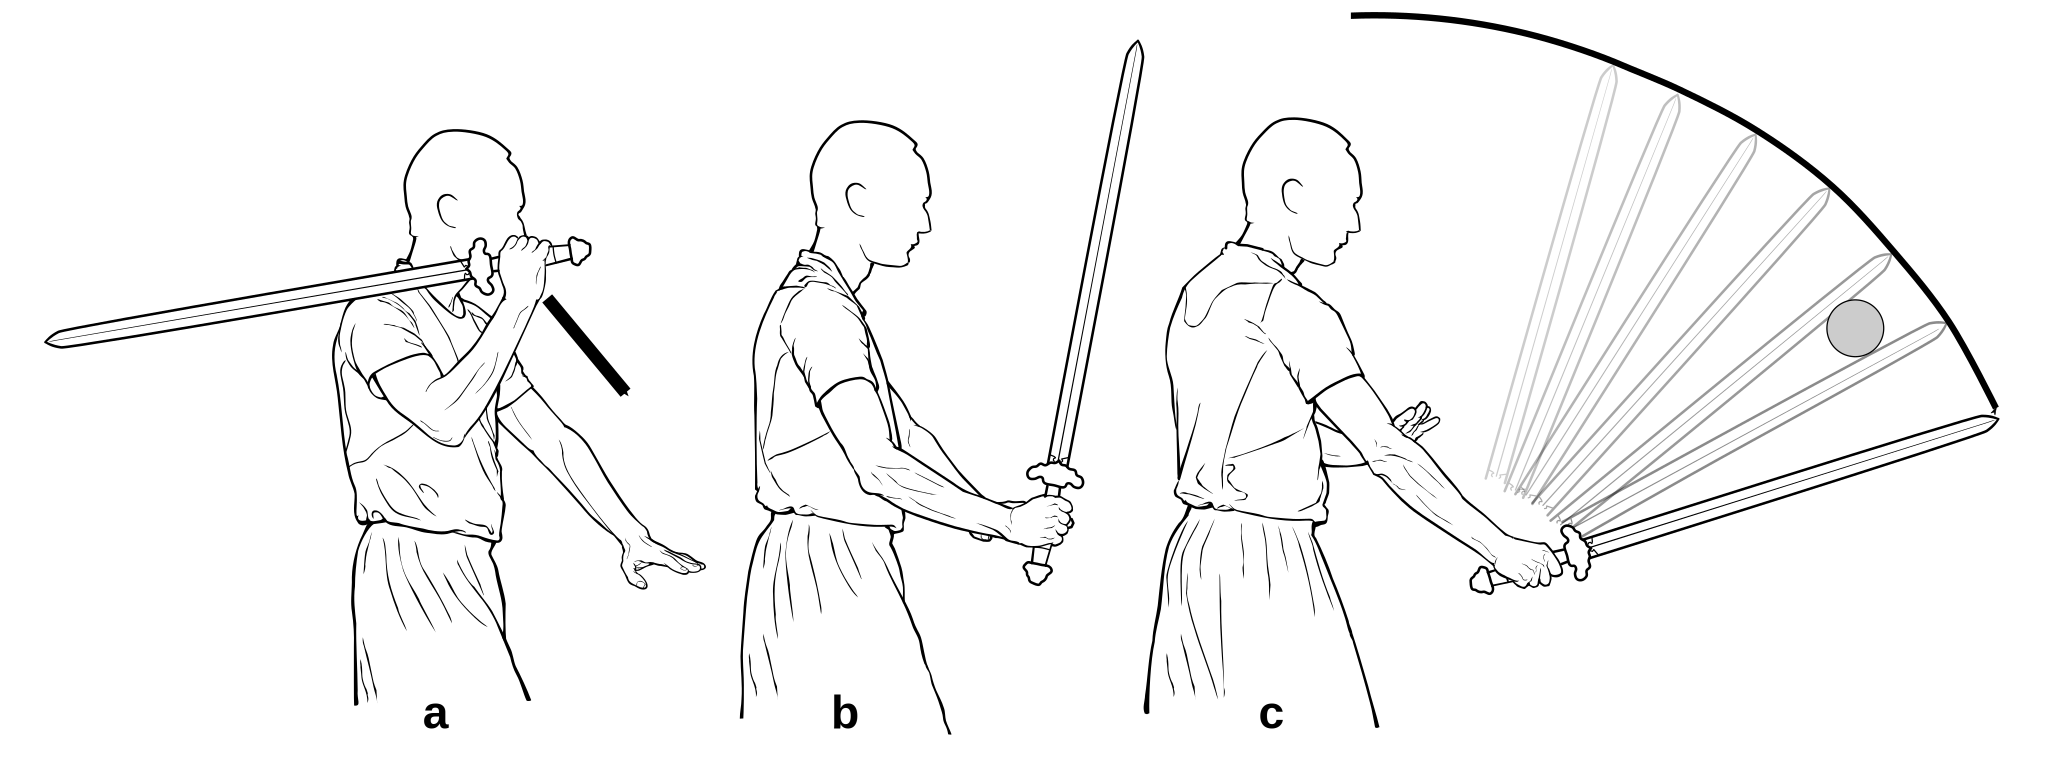
\includegraphics[width=1.00\textwidth]{../../Images/JibenJianfa/Pi/Pi_juxtaposed.pdf}
	\caption[\Pi{} cut]{\Pi{} cut: (a) Starting from a high position of the sword, the right hand draws the sword handle downwards to accelerate the blade; (b) shows the end of the acceleration phase, from now on, the hand will not exert any more action on the handle; (c) the hand follows the handle with only a firm control of the sword's trajectory so that the blade is allowed to move freely though the target represented here by a grey circle. Note that the trajectory of the blade tip is not circular but an elongated arc.}
	\label{fig:pi_cut}
\end{figure}

It is absolutely crucial that the flat is perfectly aligned with the blade trajectory to make sure that the weight of the blade lies behind the edge to push it through the target. If the blade hits the target at an angle, no matter how small, it tends to rotate on its axis and may bounce back dangerously instead of nicely cutting through the target. On the other hand, when the alignment is correct and the grip is relaxed, the blade will flash through the target without any appreciable feedback. 

After the cut, the handle naturally presses against the heel of the hand and all the fingers tighten their grip to bring the sword to a halt at waist level in a protective position without any tension nor bounce. Thanks to a proper body alignment, the sword's energy is thus returned to the body, helping to recentre oneself and make ready for the next technique.

\fiche{ 
training tips and drills
figures: the whole technique,  blade alignment with trajectory

combination of the  sword rotation and the forward movement of the hand.
unwinding movement with extension to the front like angling but with a downward direction as well.
splitting,  short,  often done at the beginning of other cuts such as Hua generally performed in a downward direction, but may be oriented towards any direction 
}

\section{\Hua}
The verb \Hua{} \begin{CJK*}{UTF8}{bsmi}劃\end{CJK*} means \textit{to delimit}, \textit{to draw}. The same character is also used as a variant of the word for an individual stroke in a Chinese character. 
Along with the fact that the left part of this character is indeed the key for the brush, these observations tend to suggest that the technique somehow evokes the notion of calligraphy, of writing or drawing. 

The emblematic technique is presented in the \Yangjia{} \Michuan{} as a horizontal cut or a large horizontal movement for keeping opponents away. The idea is here to sweep space with the sword to delimit the largest possible area around oneself and slash anyone closing in. 

In a more general perspective, \Hua{} cuts do not need to always be horizontal and encompass a whole range of distances, from very long slashing cuts with the very tip of the blade, to very close-range drawing cuts with the whole edge. In any case, all \Hua{} cuts have in common to be long-energy slicing movements where the blade actually draws a groove in the target instead of splitting it open at once like the short-energy \Pi{} cut does. 

When performing a long-range \Hua{}, the sword is thrown forwards and, when the arm has nearly reached its full extension, slightly before the blade hits the target, the grip is gently tightened to secure the connection between the centres of the sword and the body. The rotation thus continues around the shoulder while the sword is pulling the body forwards until maximal reach is achieved (fig. \ref{fig:hua_cut} a-c). Then, the grip acting as a fulcrum, the sword's inertia pushes back the handle against the heel of the hand. This results in a slicing cut and a backward movement that centres the body back into a guard stance (fig. \ref{fig:hua_cut} d-f).

\begin{figure}[ht]
\centering
	\includegraphics[width=1.00\textwidth]{../../Images/JibenJianfa/Hua/Hua.pdf}
	\caption[Long-range \Hua{} cut]{Long-range \Hua{} cut: (a) Starting from a high position of the sword, (b) the right hand throws the pommel forwards; (c) shows the end of the active phase of the technique; (d) to (f) during the passive phase, the sword's inertia pushes the hand backwards, performing the slicing cut and centring the body back into position.}
	\label{fig:hua_cut}
\end{figure}


At closer range the dynamics of the \Hua{} cut rely less on sword's inertia but more on body structure and movement. Once the edge of the blade is in contact with the target, the slicing cut is generated by pressing the edge against the target while pulling it in a direction parallel to the blade, either with a step or a rotation of the body. On some occasions, in particular when one is passing behind the opponent's back, it may be possible to perform a short range \Hua{} with the false edge. 

Beside being a slicing cut, \Hua{} can also be used to keep the opponents at distance or to incite them to react so we may exploit their action and take control of the rhythm. This is achieved either performing an uncommitted long-range \Hua{} or whirling the sword while advancing. This should definitely be done at a distance close enough to be perceived clearly as a threat even though we may be out of measure when doing so. The ideal distance is actually the very upper limit of the short measure, at which distance, a hit being uncertain yet perfectly plausible, the opponent will feel compelled to react defensively. It is crucial here to get ready to follow up with a more committed attack or with a blade control depending on the opponent's reaction. This second intention will thus ensure to keep the initiative and exploit the opponent's action.

\fiche{
This does not mean though that we must have a predetermined second action in mind, but that we should abandon the initial intention of the \Hua{} and prepare to transform and adapt to the opponent's reaction as soon as they start parrying. This combination of our first uncommitted attack with a timely transformation into a second action while the opponent is just starting to defend against the first one ensures we are one time ahead and keep the initiative. But this definitely requires a state of awareness to avoid an inappropriate action which would allow the opponent to retaliate while we are unprepared. Even though we have taken the initiative, we must none the less conform to the opponent's actions. And we must feel instantly whether the situation is not suitable for a second attack or a riposte, and then withdraw into a safer position out of measure. 
}

While withdrawing after an unsuccessful attack, we may want to keep our opponent away with a series whirling cuts performed in a row, which Master Wang Yennien described as being \Hua{} cuts as well. This application of the technique perfectly fits the translation \textit{to delimit} as it creates indeed a zone of security and prevents the opponent from catching up and attacking us while we are getting out of measure. 

\fiche{
is the principle of the relationship between the centre of the sword and the body.
related to calligraphy: trace a line with the point of the sword thanks to the unity achieved between the sword and the body
NO THE PRINCIPLE OF CONNEXION IS INCLUDED IN SI YAO
the movements of the body are transmitted to the point of the sword which traces lines in the air
}

\section{\Ci{}}
The word \Ci{} \begin{CJK*}{UTF8}{bsmi}刺\end{CJK*}, which means \textit{to thrust}, \textit{to pierce}, \textit{to stab}, is used in the \WubeiZhi{} as a generic term referring to all thrusting techniques. It is mentioned as well in other ancient treatises to describe thrusts with a variety of weapons.

In the \Yangjia{} \Michuan{} tradition, \Ci{} can be defined as a powerful upward or horizontal thrust where the point is pushed forcefully through the target. 

The formal technique is habitually performed starting on the right foot, left leg forward, either with a passing step (long \Ci{}) or with a simple transfer of the weight onto the left foot (short \Ci{}). In the formal context of drills and routine practice, the short \Ci{} is aimed at the belly and the long one at the throat. When sparring though, other parts of the body, such as the torso or even the face, are also targeted.

Long or short, the technique invariably starts by creating in the body a spiral structure connecting the left foot to the sword. As soon as the waist starts moving, the right arm pushes on the handle and rises in a spiralling movement that ends up with a flat horizontal sword position, the pommel oriented towards the left hip. Simultaneously, the weight is transferred onto the left foot. The grip gradually adapts to achieve a uninterrupted connection between the hand and the handle, without any kink, suitable for pushing the sword forwards effortlessly. The adjustment of the grip also permits the exertion on the handle of an oblique action reaching through the guard for a point just beyond to generate at the tip a pivot point that stabilizes it\footnote{See chapter \ref*{ch:chinesesword} for more details on pivot points.}. 

In the long version of the technique, a greater reach is achieved thanks to a passing step of the right foot. The right arm must be extended before stepping forward in order to improve the precision of the thrust and to keep the body as far as possible from danger behind the sword. Further protection can also be achieved by binding the opponent's blade to control it with the guard or the forte.

\begin{figure}[ht]
\centering

	\includegraphics[width=1.00\textwidth]{../../Images/JibenJianfa/Ci/Ci_thrust_arc.pdf}
	\caption[Long \Ci{} thrust]{At the end of the long \Ci{} thrust, the sword is aligned with the left hip but its point is centred, aiming at the base of the throat. The power of the whole body structure is concentrated into the sword to forcefully push the tip through the target.}
	\label{fig:ci_thrust}
\end{figure} 

Ideally, the right heel should touch the ground exactly at the same time as the blade tip reaches the target. The relaxation of the structure then completes the passing step while pushing the blade through. While doing so, it is important not to fall into the right leg to keep our ability to withdraw quickly if needed. This does not mean though that the weight should not be in any way transferred onto the right leg, but that the polarity empty/full between the two legs should be maintained under all circumstances so as to avoid double weight. A powerful yet mobile structure is thus achieved by the generation of an arc of force, going from the left foot, traversing the back, spiralling along the right arm to reach the tip of the blade, and backed up by the spiral in the left arm and sword fingers.

Besides the above emblematic form, the \Ci{} techniques may encompass other powerful thrusts leveraging the body structure to push the sword forwards in a, clockwise or anticlockwise, spiral. In all those techniques, a protective cone is created,  whose point aims at the target and within which one can step in, safely hidden behind one's own sword. 

\fiche {
figures: 1 hand position, spiral path in the whole body,  protection arm extended

3 the protective angle of the guard is increased when it is farther from the body

This way of controlling the opponent's blade bears some similarity to the capturing of the opponent's blade with the guard mentioned in the Principles of the Wudang sword.
It should be noted here too that this kind of control is entirely consistent with the fact that the tip is a pivot point when applying a force on the blade near the guard of a properly balanced sword. This ensures indeed that the contact of the opponent's blade has virtually no effect on the tip and does not prevent it from staying in line with the target when thrusting. 
}


\section{\Duo}
The translation of \Duo{} \begin{CJK*}{UTF8}{bsmi}剁\end{CJK*}, referring to the cooking term \textit{to mince}, somehow suggests repetition and cutting using a part of the blade further away from the tip than \Pi{}. The movement itself is a combination of a forward extension with some sort of shearing, as if using a large cooking knife to mince herbs or vegetables.

In the \Yangjia{} \Michuan{} tradition, the emblematic \Duo{} is performed with both arms extended almost in line with the sword's blade (fig. \ref{fig:duo_full}). 


\begin{figure}[ht]
	\centering
	
	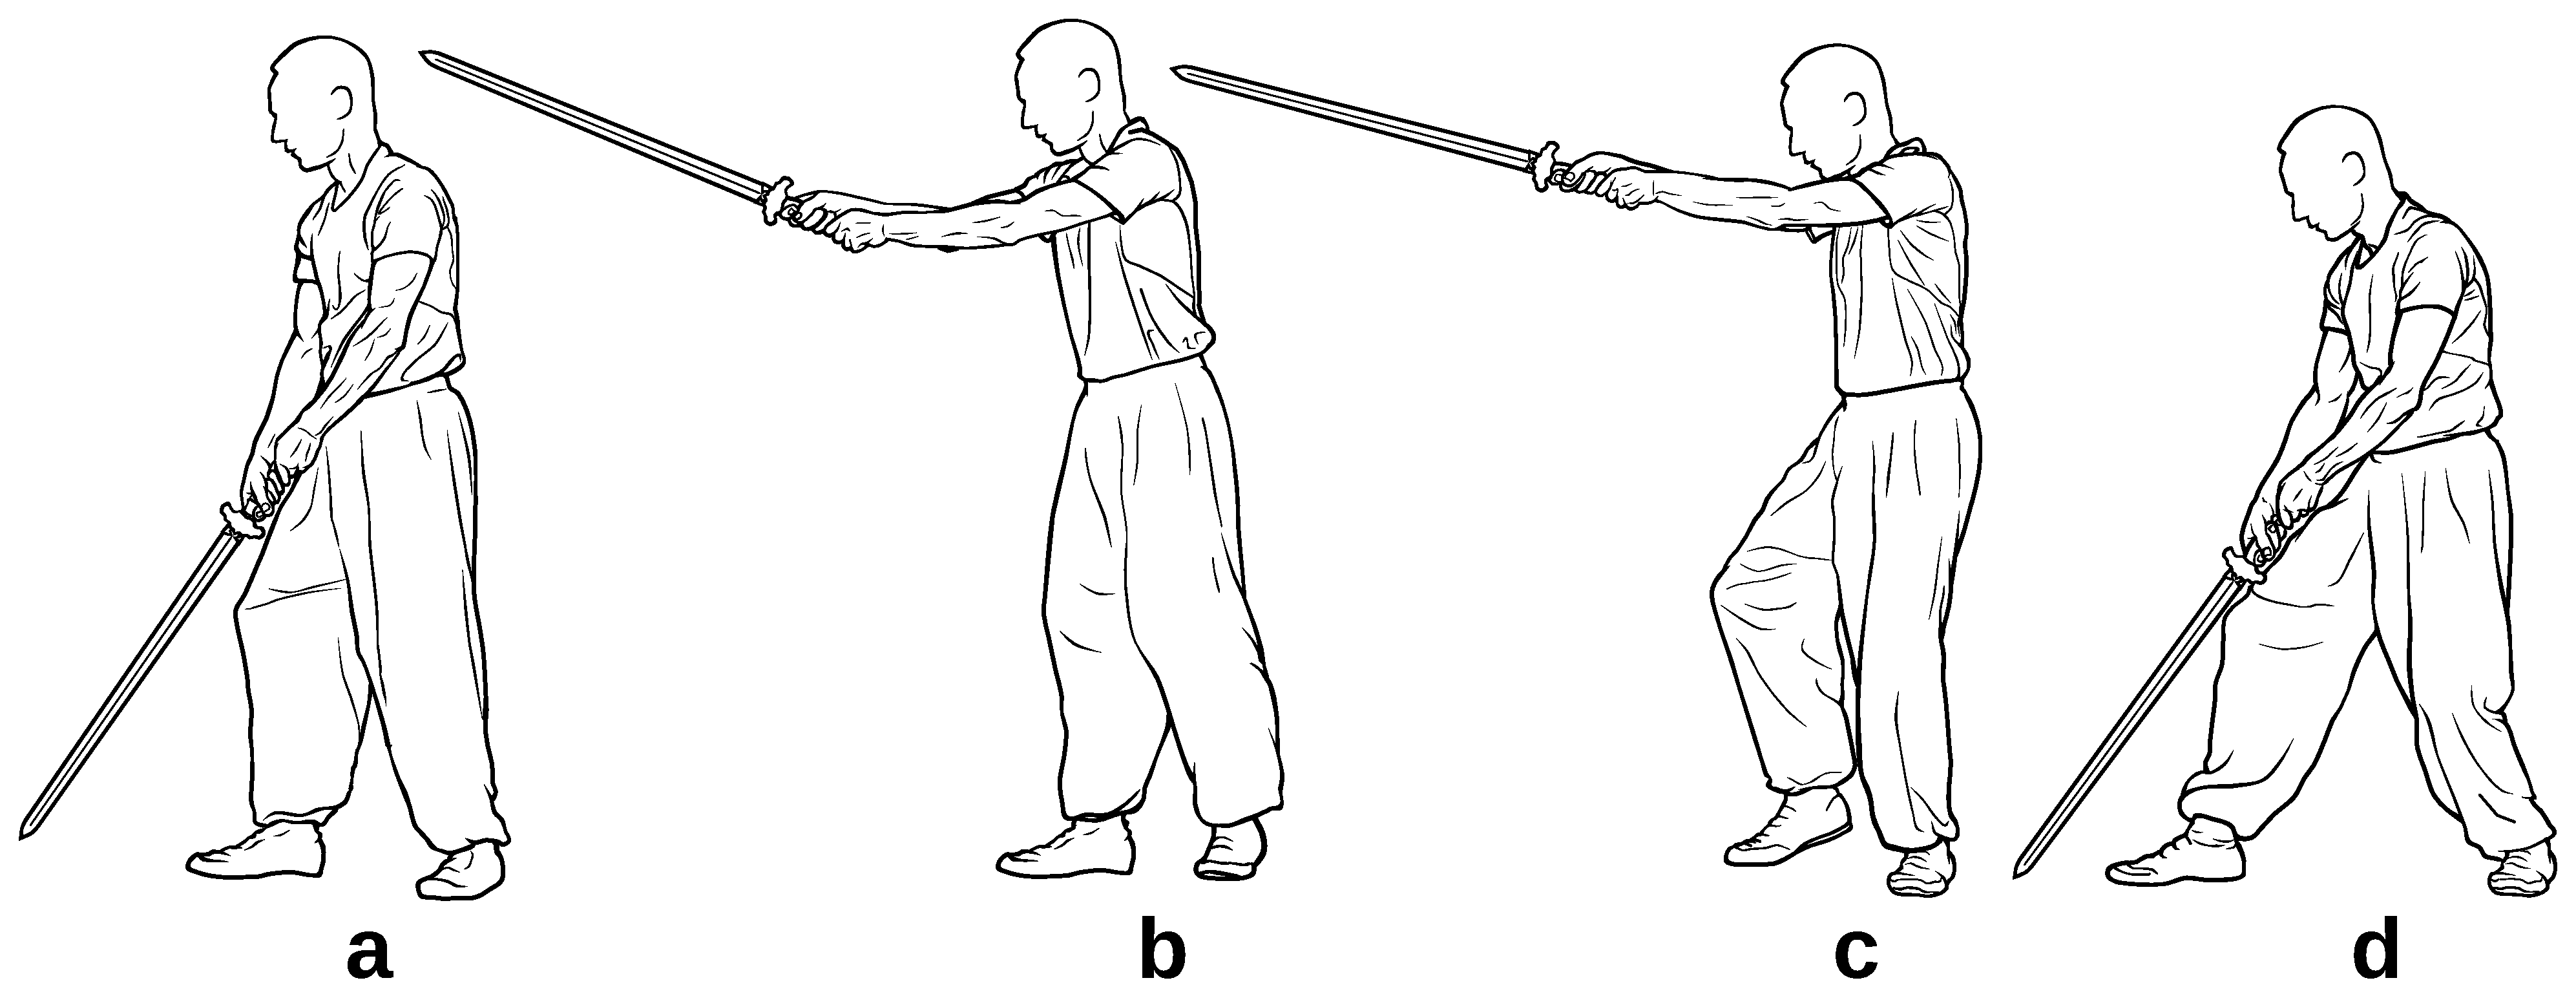
\includegraphics[width=1.00\textwidth]{../../Images/JibenJianfa/Duo/../Duo/Duo.pdf}
	\caption[\Duo{}]{\Duo{} in the forward direction. From a low guard (a), raise the sword with a transfer of the weight onto the right foot (b), invert polarity and transfer the weight back onto the left foot (c), drop the sword while sinking in the left leg and advancing the right foot.}
	\label{fig:duo_full}
\end{figure} 

Even though both hands are in contact with the handle,  this should not be mistaken for a true double handed grip of the sword. The right hand holds the sword while the left hand provides the structure and power coming from the waist by acting on the pommel along the direction of the blade. The combination of the right hand's passive role with the left hand's action creates a polarity resulting in a movement of the sword perpendicular to the axis of the right arm (fig. \ref{fig:duo_detail}). 

\begin{figure}[ht]
	\centering
	
	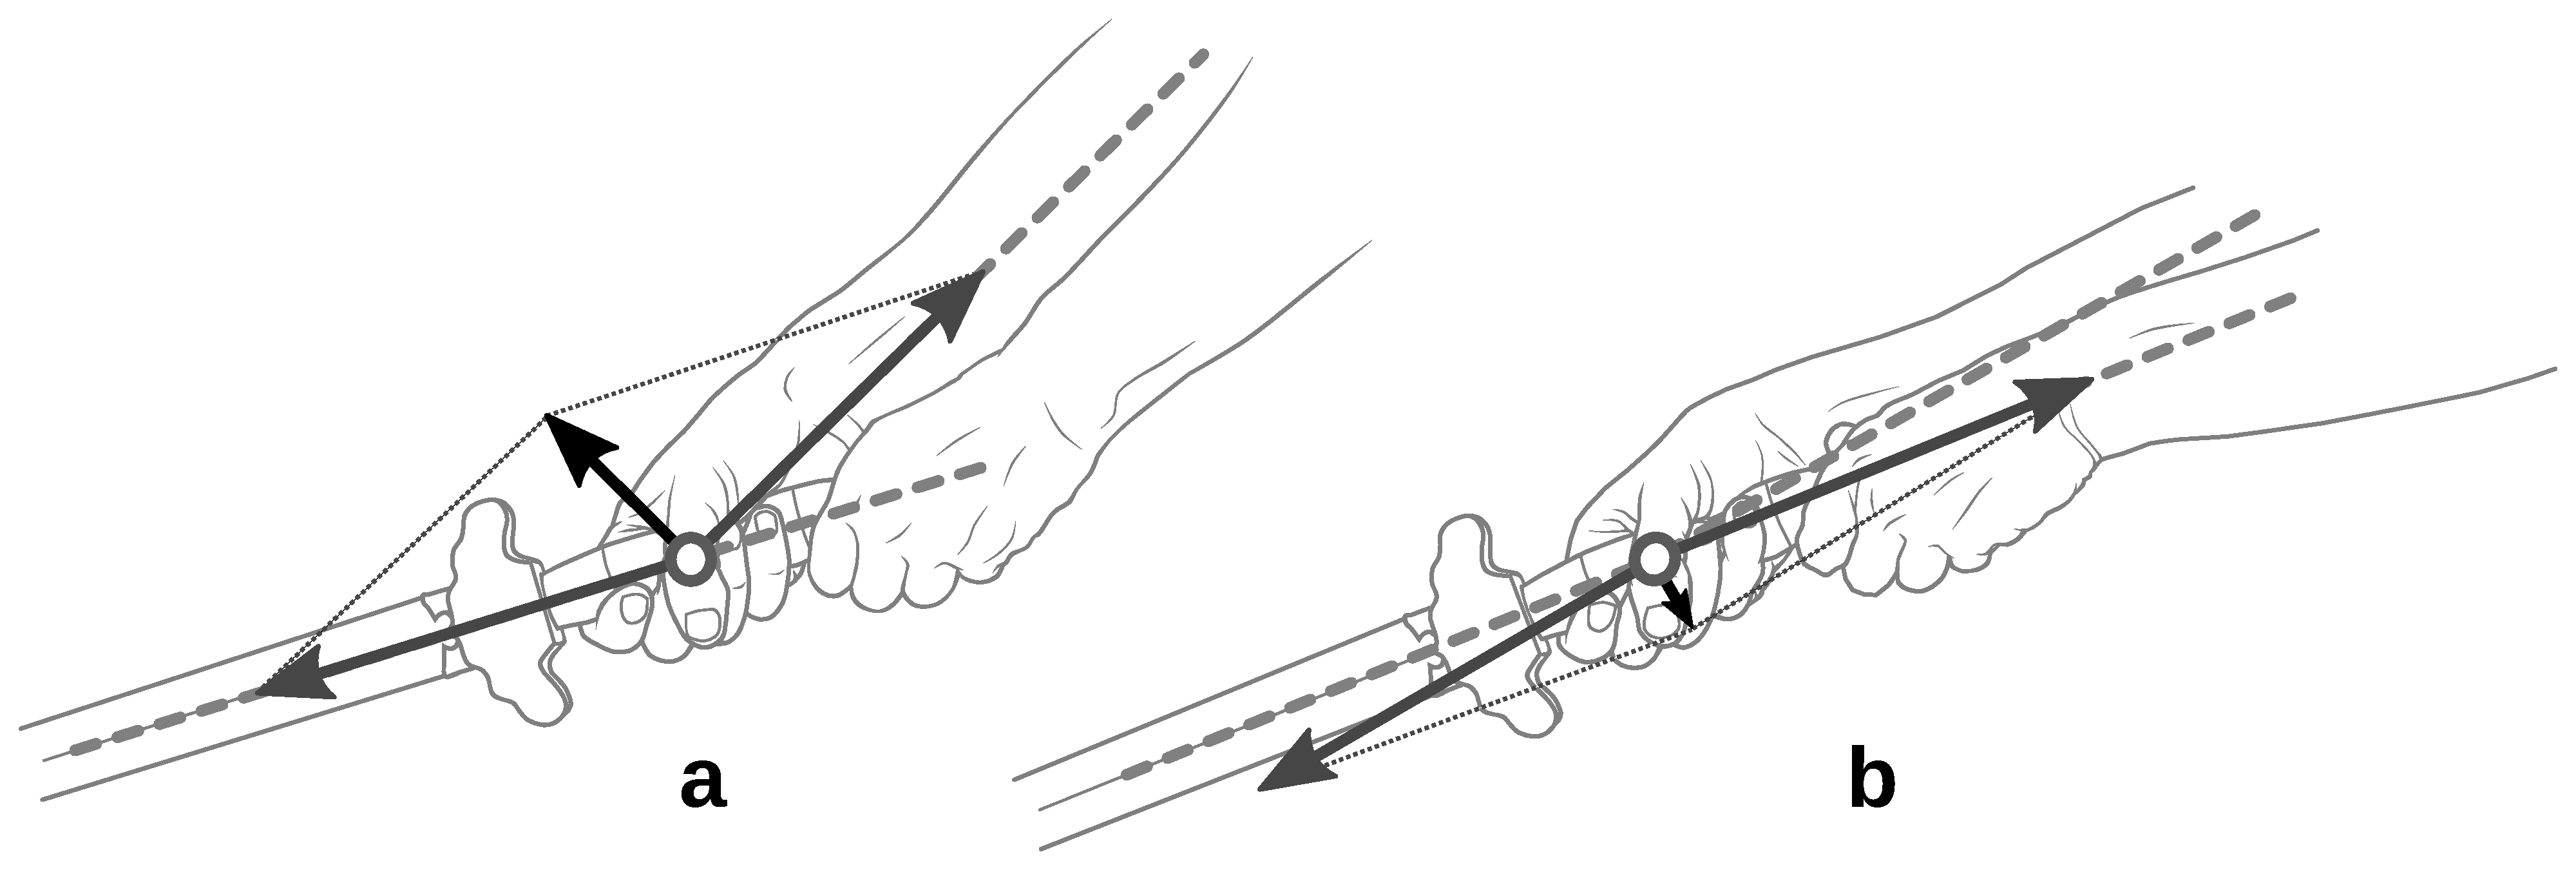
\includegraphics[width=1.00\textwidth]{../../Images/JibenJianfa/Duo/../Duo/DuoDetail.pdf}
	\caption[Balance of forces in \Duo{}]{(a) To perform a rising \Duo{}, the left hand pushes the handle in the direction of the blade tip while the right arm passively balances the pushing force. Due to the angle between the pushing direction and the right arm, the resulting force perpendicular to the right arm pushes the sword upwards in a circular movement around the right shoulder.\\
	(b) To perform a descending \Duo{}, the left hand pulls the handle while the right arm passively balances this force. The resulting force draws the sword downwards in a circular movement around the right shoulder.
	}
	\label{fig:duo_detail}
\end{figure} 

The power of \Duo{} thus originates in the weight transfer from one foot to the other, is transmitted to the sword by the left/rear hand with the right/fore hand exactly and passively balancing the forces to effortlessly generate the technique. An effective connexion between the waist and the sword will allow the explosive expression of the \Duo{} technique. 
This method somehow echoes the precepts found in the \JianJing{} stating that, when wielding a double-handed sword, power is first in the waist, then in the rear hand, and finally in the fore hand.

Since, when cooking, herbs are usually minced by cutting downwards, we may argue that the active phase of \Duo{} is the descending one. However, if we examine attentively the actual movement of a kitchen knife when mincing, we may discover that its form when cutting actually corresponds to the rising phase of \Duo{}. The main difference is that the tip of the knife stays down in contact with the table whereas the point of the sword rises up. But, in both cases, the edge follows the same movement relative to the tip. 
However, it is perfectly possible to be active in both phases, the actual passive phase being the transition movement between the ascending and descending parts of the technique. Thus, \Duo{} can be a raising thrust or cut as well as a descending cut, or, combined with \Mo{} energy, an action on the opponent's blade, either ascending to intercept and deflect or descending to shear. 

It is worth noting at this point that, since both hands are in contact with the handle, the sword is always in line with the axis of the body. This axis is more to the left when we are on our left foot, in the low on-guard position that precedes the ascending forward phase of \Duo{}. Reciprocally, the axis is shifted to the right as we stand on our right foot after we have completed the ascending forward stage of the movement. This has strong implications on the deflect/shear application of  \Duo{} in combination with \Mo{}. Deflecting while transferring the weight to the right gently pushes the opponent's tip away, then, the descending shear naturally aims at the centre of the opponent's sword, deflecting it further to open the way for a hit while preventing any counter attack. 

\fiche{The simplest application of \Duo{} starts with a lower guard as an invitation for the opponent to prepare an attack. We can then engage and deflect with a \Duo{} before placing our riposte or we may take advantage of the explosive nature of the movement and use an offensive \Duo{} to thrust directly during the opponent's preparation.
\Duo{} is often performed in series of two to three movements, not more to avoid predictability, as seen for the double-handed version in the \Kunlun{} form. We can usually identify three periods in these series: The first \Duo{} movement would intercept an incoming attack, either a \Pi{} or a \Hua{} cut from above or a high level \Ci{} thrust.Then, the second one will deflect the opponent's blade to open the way for the third \Duo{} thrust. Of course, this is not a fixed pattern, and the first movement can be followed by any appropriate technique depending on the circumstances. For instance, instead of deflecting, the second step may accompany the opponent's blade to control it while entering to prepare the riposte.}

Although the classic movement is done with two hands, it is also possible to perform a \Duo{} with one hand only. In this case, the heel of the right hand plays the role of the left hand and the first three fingers \textemdash{} the index and middle fingers, and the thumb \textemdash{} play the part of the right hand (figure). 

During the ascending phase, the handle of the sword is pushed forwards by the heel of the hand and simultaneously pulled by the first three fingers. Given a good structure in the on-guard position, it is then possible, even with only one hand, to swiftly and effortlessly raise the sword from a low to a high position, for thrusting or engaging.  
\fiche{When descending, the fore fingers relax their grip while the ring and little fingers are tightened to pull the handle. Some intention should be put at the base of the index to gently push the handle downwards in the forward direction. The resulting structure allows to capture and deflect the centre of the opponent's sword by shearing or to perform a powerful cut while retreating.}
The alignment of the sword is quite similar to the two-handed version, with the tip of the blade in line with the body axis. However, the structure is not as strong as in the two-handed \Duo{} and, as a result, the shearing actions are not as powerful. However, this version of the movement is useful for quickly engaging the opponent's blade or a sudden attack from a lower guard. 

\fiche{
These actions can be chained, as in the \Kunlun{} sword form, by two or three, first intercepting the opponent's blade before deflecting and hitting with a double or treble shearing. 
the polarity between the hands allows the crossed links between hand and foot. 
}

\section{\Liao{}}
Translating as \textit{to raise}, \textit{to lift}, \textit{to sprinkle}, \Liao{} \begin{CJK*}{UTF8}{bsmi}撩\end{CJK*} is found in various ancient manuals for different weapons. The \Yangjia{} \Michuan{} tradition describes the technique as an upward cut, but it is sometimes also considered as a defensive action used to parry or deflect an incoming attack. Technical details will vary according to the type of cut performed, splitting or drawing upward cut, or whether \Liao{} is used to parry.
All variations though have in common the upward direction of the movement, as if raising a curtain, which may explain the fact that this character has the key for the hand instead of the knife.

In the \Yangjia{} \Michuan{} tradition, \Liao{} cuts is usually presented in series of two consecutive cuts, one from left to right then one from right to left.  

\fiche{
Starting on the left leg with the right foot forward and the sword in the left lower line, the weight is shifted onto the right foot with a rotation of the hips, which gives the initial impetus to the sword. Then, power is released, raising and accelerating the sword with an expansion of the body and a forward extension of the arm. The blade follows a slanted trajectory from the lower left to the upper right line, sliding along the target, or traversing it in the sagittal plane in the case of a splitting cut. When performing a splitting \Liao{}, just as was described for \Pi{}, once the sword's centre of gravity has passed the hand, no more action should be exerted on the handle to let the sword fly freely through the target. The body should be relaxed to follow the sword, get the energy of the sword back after the cut and recentre oneself in a ready position.

From this position it is possible to let the sword continue its movement backwards down to the lower right line while passing the left foot forward, to prepare a second \Liao{} from right to left. In order to do the second cut, the weight is first transferred onto the left foot, then the rotation of the waist draws simultaneously the sword and the right leg forward. The blade thus follows an oblique trajectory from lower right to upper left either slashing or splitting the target.

Variants of the above cuts exist that are done with a sidestep to dodge an incoming attack while raising the sword to intercept the opponent's arm. The resulting cut is thus performed laterally rather than in the sagittal plane as described above. 

An extreme case of such a lateral \Liao{} cut is performed entirely in the frontal plane, from left to right. It starts first with a rotation of the waist to the left to evade or parry an attack while preparing the cut. This can be done either in place or with a crossing step to adjust for distance and direction. In both cases we end up facing left, with the opponent at our right. Swinging the sword rightwards while crouching will then aim a \Liao{} cut at the opponent's arm, groin, etc. It is important that the body should be turned slightly towards the right  when crouching so that the right shoulder is not restrained and the sword can be raised high enough to reach and split the target efficiently. 

\Liao{} can also be used for parrying and, as a matter of fact, the \Liao{} cuts described above can all be preceded by a \Liao{} parry to deflect or raise the opponent's blade out of the way. Whereas deflecting involves hitting the opponent's blade away, a softer engagement allows to gently control and guide the opponent's sword upwards while keeping our point towards their face to prepare the riposte. In this case, we get contact first with a \textit{receive} technique, then raise the sword and follow the incoming attack. The contact of the blades is crucial here to guide the correct positioning of the body and prepare the riposte conforming with the attack with minimal risk.
\fiche{ It is worth noting that for some styles, \Liao{} refers exclusively to this type of raising the opponent's sword aside and does not involve cutting in itself. (check that with Mattias)}
}

\fiche{
	It is more difficult as well to gather the energy back directly, but actually we can play with gravity which will help slowing or stopping the sword in a high position from which we may start a new technique by letting the sword go with its own weight and momentum,  using its centre of gravity as a fulcrum. 
	check where is the cut located depending on the inclination of the movement
	
	The energy generating the movement comes from the expansion of the body and waist rotation.
	This is more apparent when performing \Liao{} in a standing position, which needs less to rely on the recycling the sword's inertia after the previous move.
	
	the body is drawn forwards, the foot follows the sword with some delay. The whole movement is actually a centring passive action. The sword does the job
	
	combination of a splitting upward cut followed by a drawing cut. During the latter,  
	when cutting behind, there is only a splitting cut
	the raising m  ovement may be combined with either a splitting cut or a drawing cut
	crouching only splitting type (not quite sure as it may depend upon the distance)
}


\section{\Zha}
\Zha{} \begin{CJK*}{UTF8}{bsmi}扎\end{CJK*} is a downward thrust.
\fiche{
	spiralling arc on the outside, from the foot to the point, passing through the back and the outside of the arm and along the true edge. The back is stretched and the breast is relaxed. There is a connection between the foot and the point. The weight of the body and the rotation of the waist inwards will generate the thrust. The arm extends in coordination but not excessively
	The unarmed hand can control the opponent's arm, especially when chained after parrying \Liao{}.
	
	check the translation and make sure to use the simplified character
	translation: set up (a tent)
	
	rem: there exists another character which is simplified into this one and is pronounced at the first tone and means
}


\section{\Mo}
\Mo{} \begin{CJK*}{UTF8}{bsmi}抹\end{CJK*} encompasses all the techniques that take control of the centre of the opponent's blade.
\fiche{
	principle of controlling, deflecting, directing, listening
	the intention is located closer to the forte
	
	translation: put, spread (butter, etc.), wipe
	use the simple character
	
	maybe related to a variety of techniques used to parry, such as wash, shave, shear. ..
	
	radical mo is probably phonetical although it means powder (waste, residuals)
	
	sliding contact of the blades (wipe) with a deflecting action of control thanks to the opposition of the forte against the feeble of the opponent,  this is found in blade capture (coulé, opposition, ...) or the control of the blade during attacks
	
	lateral and aiming at the centre of the opponent's blade, if only lateral we give way to transformation by the opponent and we don't have control of their blade. 
	
	relationship with feeling through the blade and cover
	during parries, absorption, deflection, protection
}

\section{\Tiao}
\Tiao{} \begin{CJK*}{UTF8}{bsmi}挑\end{CJK*} means to rise, to provoke something or someone, to poke the fire. It is a swift cut performed with the false edge. 
\fiche{
complementary to \Dian{}
whipping movement, cut with the false edge using the centre of gravity as a fulcrum and aiming at the wrist, the fingers or the forearm
can also be an interception,  quick deflection
the sword is drawn backwards by the movement of the waist which comes back into place. when stopping, the handle is kept in place by the hand and the point of the sword rises thanks to the sword's inertia
translation: rise, provoke something or someone, poke the fire? 

}

\section{\Dian}
\Dian{} \begin{CJK*}{UTF8}{bsmi}點\end{CJK*} is a swift thrust or light cut performed with the very tip of the blade.
\fiche{
fast thrust thrown in a light fast way like a jab
can also be a quick light cut aimed at a forward target such as the wrist
translation: drop, strain, point, aspect
mark with a dot, touch lightly, instill, count, choose, suggest, light up, 
a little, hour
complementary to\Tiao{}
}

\fiche{
\section{What makes a cut effective? }
relaxation, blade alignment
distance
must travel through the target
split or slice

\section{ What makes a thrust effective?}
point control, see pivot points in chapter 2
distance
no need for more than a few centimetres in the target to reach a vital organ
}
